\section{Introdução}

Classificação morfológica é o agrupamento de galáxias conforme sua forma. Como esta classificação é baseada na inspeção visual das imagens, elementos subjetivos são agregados. Em 1926, o astrônomo Edwin Hubble, na tentativa de relacionar a origem das formas das galáxias sistematicamente, criou o método hoje conhecido como \emph{Hubble Sequence} ou \emph{Tunning Fork}. \cite{hubble1926, fortson2012}

\begin{figure}[h!]
  \centering
  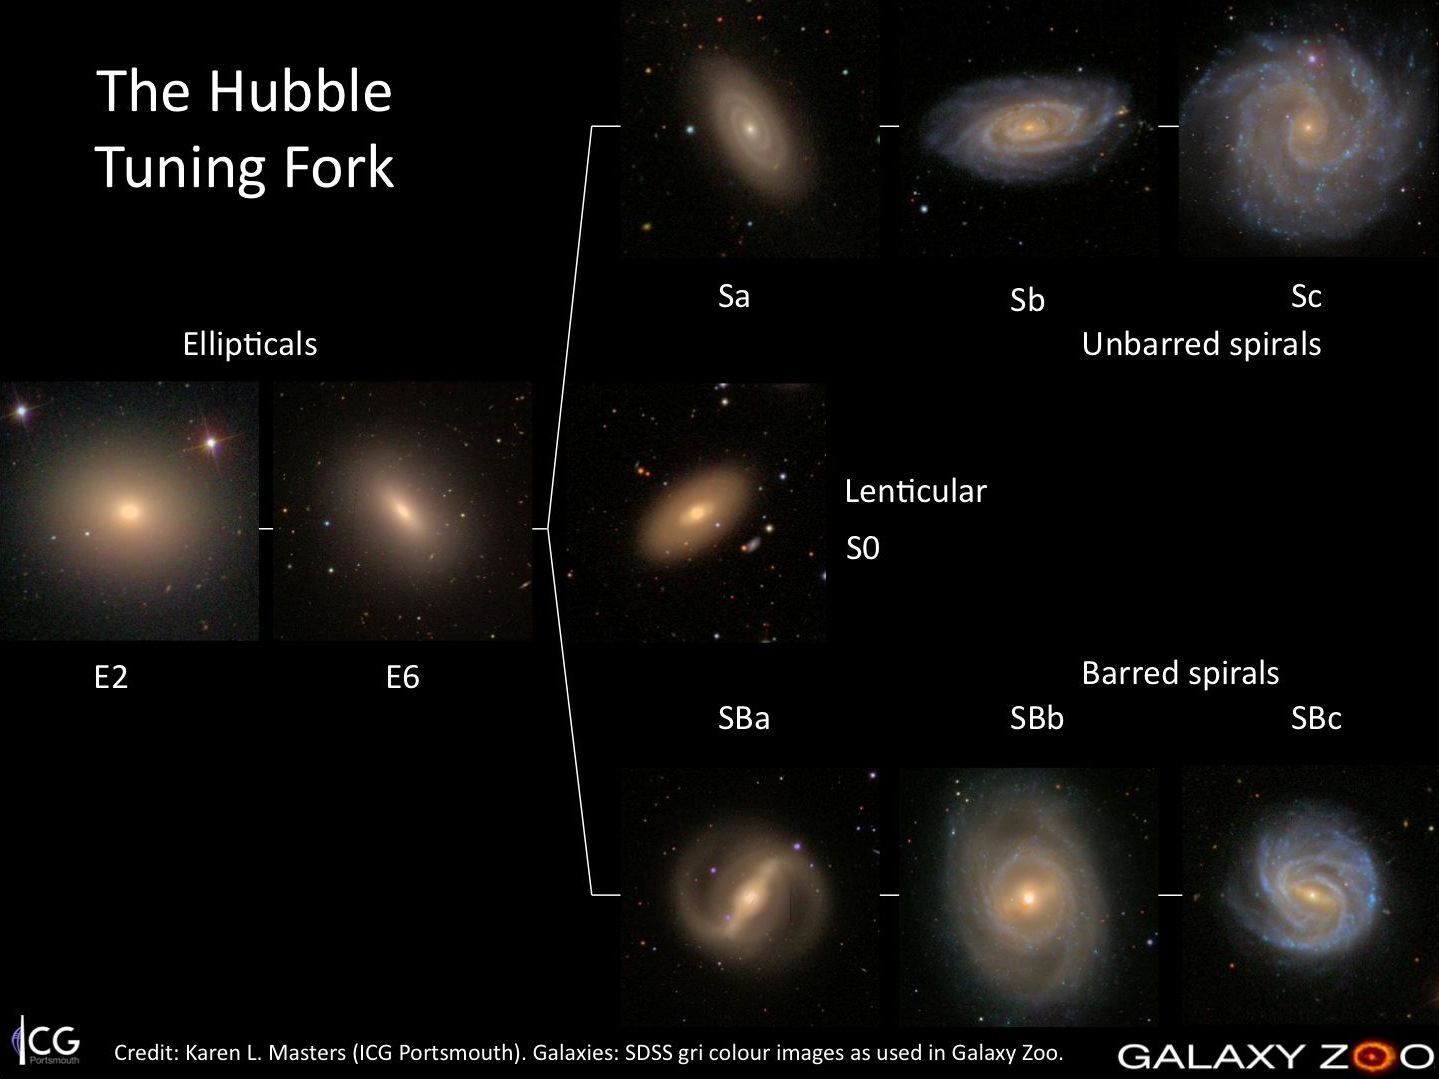
\includegraphics[width=.8\textwidth]{figures/tuningfork1.jpg}
  \caption{Diagrama da Sequência de Hubble.}
  \label{fig:tuningfork}
\end{figure}

As formas predominantes de grandes galáxias na natureza são elípticas e espirais. A figura \ref{fig:tuningfork} mostra um esboço da atribuição de classes discretas às galáxias de acordo com suas formas. Nela as galáxias são classificadas como elípticas, espirais ou lenticulares. \cite{fortson2012}

O GalaxyZoo\footnote{https://galaxyzoo.org.} é um projeto \emph{citizen science} realizado com auxílio de cidadãos, a maioria sem vínculo acadêmico, que contribuem com seus conhecimentos e observações. A segunda liberação de dados do GalaxyZoo possui um catálogo com classificações morfológicas de trezentas mil imagens de galáxias do SDSS\footnote{SDSS: Sloan Digital Sky Survey -- https://www.sdss.org.} feitas por voluntários e acuradas segundo o método de Hart et al. \cite{hart2016}

Com o avanço dos levantamentos (\emph{surveys}) digitais, é substancial a criação de métodos rápidos e automatizados para a classificação morfológica de galáxias sem a perda da acurácia da tradicional classificação visual. \cite{yamauchi2005} O uso de \emph{Deep Learning} tem mostrado bons resultados e as Redes Neurais Convolucionais são ferramentas de grande potencial para processamento de imagens. \cite{barchi2020, dai2018}

O S-PLUS \cite{oliveira2019} é um levantamento de galáxias do espaço local com um telescópio construído no Chile e a Universidade de São Paulo como uma das instituições fundadoras. A parte do mapeamento que cobre a região do chamado \emph{Stripe-82}\footnote{É um campo equatorial do céu de 300 graus$^{2}$. Cobre a região com ascensão reta das 20:00h às 4:00h e declinação de -1,26$^{\circ}$ a +1,26$^{\circ}$.} foi concluída recentemente e existem muitas informações a serem exploradas. Diariamente o telescópio gera uma enorme quantidade de dados, daí a importância de técnicas automatizadas para o processamento destes.
